
\section*{a. State-of-the-art and Objectives}

\subsection*{1. Background}

\smallskip
\smallskip
\noindent
In the local Universe, there is a link between the key properties of
massive galaxies, such as bulge mass, and their central supermassive
black holes 
%(SMBHs; e.g., [1], [2]). 
\citep[SMBHs][]{KormendyHo2013, Kormendy2016}
This has led to the proposal that
the supermassive black hole, when accreting, has an influence on its
host galaxy by the means of some regulatory ``feedback'' mechanism(s)
\citep[e.g., ][]{AlexanderHickox2012, Fabian2012, KingPounds2015}
%(e.g., [3], [4]). 
However, the details of the physical processes
involved in AGN feedback are still disputed
and, moreover, direct observational evidence for AGN feedback in the
early universe is conspicuous by its absence 
\citep[e.g., ][]{HeckmanBest2014, NaabOstriker2017}
%(e.g., [5], [6]). 
Hence, a major source of uncertainty in our current
understanding of galaxy evolution is how supermassive black holes
influence, and potentially regulate, their host galaxies. 
\citep{Carilli_Walter2013, MadauDickinson2014, Netzer2015, Padovani2017, Xue2017}


\smallskip
\smallskip
\noindent
Current theories of galaxy formation and evolution now strongly
suggest that central, supermassive black holes (SMBHs) have a profound
affect on the galaxies that they live in. This is not surprising since
the potential energy associated with mass accretion onto a
supermassive black hole is comparable to that generated via the
nuclear fusion in the galaxy's stars. Thus when a galaxy goes through
a ``quasar'' phase, there is ample energy to potentially impact the
host galaxy and surrounding intergalactic medium.

\smallskip
\smallskip
\noindent
What is the main AGN triggering mechanism at the height of quasar
activity? What direct observational evidence in individual objects
links AGN activity to star formation?  Can we observe ``AGN feedback''
in action, in situ, for the most luminous sources?  Such unknowns
about the co-evolution of black holes and their host galaxies remain
among the most fundamental unanswered questions in extragalactic
astronomy.


\smallskip 
\smallskip
\noindent
Furthermore, the details of the physical processes involved in the AGN
activity including how the SMBH directly couples and affects its most
local environment, i.e., the accretion disk, broad line region and
dusty torus, are still unknown at this point (e.g., [7], [8]). Noting
- and for the most part, currently ignoring this issue - quasars have
become key cosmological probes; by being high-$z$ tracers of the
underlying matter distribution ([9]) and as ``backlights'' to observe
the IGM (e.g., [10-15]).


\smallskip
\smallskip
\noindent
However, the interaction and the details of physical processes involved in how
this energy escapes the inner most regions of the galaxy and then
interacts with the gas, dust, stars and dark matter, is currently poorly understood, 
with current observational data giving more puzzles
than clues on how to make progress. Further issues arise since startling new 
observations (e.g. MacLeod, Ross et al. 2016; Ross et al. 2018) show that {\it
quasars vary significantly on timescales of weeks to months}, whereas the
accretion disks (that are thought to supply the `fuel' for the quasar) 
should take thousands of years to change their optical emission (see
e.g. Lawrence 2018, Nature Astronomy).  Thus, it is unclear to what level we have 
an understanding of a prevalent astrophysical phenomena; the
accretion disk.


\smallskip
\smallskip
\noindent
Variability studies hold information on otherwise unresolvable regions in Active Galactic Nuclei (AGN). Population studies of large samples likewise have been very productive for our understanding of AGN
\citep{Lawrence2016_ASPC}. 
These two themes are coming together in the idea of systematic variability studies of large samples and the field of observational extragalactic astrophysics is poised for a fundamental and rapid change. 
%%
Starting in late 2019, a fleet of new telescopes, instruments and missions are coming 
online over the next few years that will leap-frog the quality and
quantity of data we have available today. Over the course of the next
5-6 years, surveys and missions including the fifth incarnation of the
Sloan Digital Sky Survey
(SDSS-V\footnote{\href{www.sdss.org/future/}{{\tt
www.sdss.org/future/}}}), the Large Synoptic Survey Telescope
(LSST\footnote{\href{lsst.org}{{\tt lsst.org}}}), the Dark Energy
Spectroscopit Instrument (DESI\footnote{\href{desi.lbl.gov}{{\tt
desi.lbl.gov}}}) survey, the 4-meter Multi-Object Spectroscopic
Telescope (4MOST\footnote{\href{4most.eu}{{\tt 4most.eu}}}) survey,
and the ESA {\it Euclid}
mission\footnote{\href{sci.esa.int/euclid/}{{\tt
sci.esa.int/euclid/}}}, will see first light. Even more imminent is
the launch of the {\it James Webb Space Telescope}
(JWST\footnote{\href{jwst.stsci.edu}{{\tt jwst.stsci.edu}}}).


\subsection*{2. Objectives}

\smallskip
\smallskip
\noindent
This proposal has two broad and well-posed goals.  
% \smallskip\smallskip \noindent
First, we aim to
elucidate in detail {\it how the energy directly associated with a
supermassive black holes impacts the universal galaxy population.}  We
will gain a deep understanding into the physical mechanisms related to
central engine black holes; their accretion disk physics, their
dynamics on both human and galactic timescales and the role they might
play in forming, and regulating the galaxy population. 
We will investigate what the observed rapid changes tell us about the SMBH and accretion discs, 
and does ``quasar feedback'' regulate galaxy formation?
{\it Ultimately, we want to discover if there is a missing link between the 
activity on sub-parsec scales that impacts on the galaxy-wide kiloparsec scales.}
These are among the most prescient astrophysical issues of our time, 
and where major breakthroughs are imminent.

\smallskip
\smallskip
\noindent
Second, we will {\it discover brand new extragalactic phenomena.}  By
tapping into the massive and raw discovery space that the new
experiments will open up, there is the highly likely outcome of
discovering something ``brand new''. The LSST will deliver a dataset
so spectacularly different both in sky coverage and time-sampling
coverage, that the Universe would have to be an exceptionally boring
place to not have brand new astronomical objects and astrophysical
phenomena waiting to be discovered.

\smallskip
\smallskip
\noindent
We will achieve this by leveraging several of the new, large-scale
surveys that are coming online in the next few years. These critical
observations are made by exploiting the large imaging and
spectroscopic datasets that we will have available from the SDSS-V,
DESI, 4MOST, LSST and ESA {\it Euclid}. {\it Crucially, although these 
projects individually will deliver new state-of-the-art datasets, it is 
our project that will be the first to break down the associated data 
silos and combine these data in order to go beyond the state-of-the-art.}


\smallskip
\noindent
Our ERC Consolidator grant proposal will radically improve our understanding of 
one of the two fundamental energy sources available to galaxies; that of accretion 
onto the compact object in the central engine. We will achieve this by leveraging 
several of the new, large-scale surveys that are coming online in the next few years. 
The scope and remit of an ERC Consolidator grant will allow us to combine these 
data products in a manner that will 
% This programme will 
not only establish the new state-of-the-art in extragalactic variable science, 
{\it it will establish and kickstart the new field of extragalactic variable science itself}. 
%%
The P.I. is a world-leader in observational quasar astrophysics, both in terms of 
survey work and individual object study. 
%%
Our proposal takes astrophysics into the 2020s, going from single objects samples, 
to surveys and samples of millions of objects leveraging these multi-billion Euro/dollar/pound  
next generation missions, telescopes and their subsequent datasets. 
%%
Quasars are ideal probes... etc. 

\smallskip
\smallskip
\noindent
Black holes are omnipresent in our Universe, and black holes that are
millions to billions of times the mass of our Sun, are ubiquitously
found at the centers of galaxies, including our own Milky Way.
Initially consider physical oddities, we now strongly suspect that
these (central, ``supermassive'') galactic black holes have a profound
affect on the galaxies that they live in. This is not surprising since
the potential energy associated with mass accretion onto a
supermassive black hole is comparable to that generated via the
nuclear fusion in the galaxy's stars.

\smallskip
\smallskip
\noindent
However, the interaction and the physical processes involved in how
this energy escapes the inner most regions of the galaxy and then
interacts with the gas, dust, stars and dark matter, is currently very
poorly understood theoretical, with very few observational data giving
insight on how to make key progress.
%
The field is poised for a fundamental and rapid change. The first data are now in hand 
that show {\it changes on human timescales} in external galaxies, with these new 
field defining studies including lead projects by the P.I. 



\smallskip
\smallskip
\noindent
In the Table below, we summarise the outstanding issues, and our novel investigations. 

\smallskip 
\smallskip
\noindent
We now know that in the local Universe, there is a link between the
key properties of massive galaxies, such as bulge mass, and their
central supermassive black holes (SMBHs; e.g., [1], [2]). This has led
to the proposal that the supermassive black hole, when accreting, has
an influence on its host galaxy by the means of some regulatory
``feedback'' mechanism(s) (e.g., [3], [4]). However, the details of
the physical processes involved in AGN feedback are still disputed
and, moreover, direct observational evidence for AGN feedback in the
early universe is conspicuous by its absence (e.g., [5], [6]). Hence,
a major source of uncertainty in our current understanding of galaxy
evolution is how supermassive black holes influence, and potentially
regulate, their host galaxies.
%%
What is the main AGN triggering mechanism at the height of quasar
activity? What direct observational evidence in individual objects
links AGN activity to star formation?  Can we observe ``AGN feedback''
in action, in situ, for the most luminous sources?  Such unknowns
about the co-evolution of black holes and their host galaxies remain
among the most fundamental unanswered questions in extragalactic
astronomy.

%%%%%%%%%%%%%%%%%%%%%%%%%%%%%%%%%%%%%%%%%%%%%%%%%%%%%%%%%%%%%%%%%%%%%%%%%%%%%%%%
%%
%%  https://tex.stackexchange.com/questions/337820/mcq-long-table-using-tikz-tcolorbox-or-tabular
%%  https://tex.stackexchange.com/questions/283419/color-in-a-multirow-cell-with-extra-vertical-space/283454
%%  https://tex.stackexchange.com/questions/406033/how-to-fit-a-cell-of-a-table-to-a-figure-and-arrange-multiple-tables/406042
%% 
%% THIS (??)::
%%     https://texblog.org/2014/05/19/coloring-multi-row-tables-in-latex/
%%
%%
%%   https://www.inf.ethz.ch/personal/markusp/teaching/guides/guide-tables.pdf
%%
%%%%%%%%%%%%%%%%%%%%%%%%%%%%%%%%%%%%%%%%%%%%%%%%%%%%%%%%%%%%%%%%%%%%%%%%%%%%%%%%


\begin{tcolorbox}[tab1, tabularx={X  X }, title=Outstanding Issues in Extragalactic Astrophysics, boxrule=1.25pt] 
Key issue                                                                            &  Novel investigation       \\ 
\hline \hline
\multicolumn{2}{c}{{\sc The physics of accretion}} \\ 
Investigating ``hot'' and ``cold'' mode accretion in the quasar population; 
determining the rates and timescales, and characterising the Changing Look Quasar (CLQ) population.   &     
Identifying and characterizing  all the CLQs in DESI and SDSS-V.  \\ 
\hline
Probing the inner parsec of the quasar central engine & 
Rapid analysis and response on LSST quasar light curves. \\ 
\hline
%%
\multicolumn{2}{c}{{\sc Obscured accretion and galaxy formation}} \\
Establish the relative importance of major mergers, minor mergers, cold streams and secular evolution 
have towards the growth of SMBHs across cosmic time. & 
Deep imaging data from LSST combined with searching for post-starburst signatures 
in DESI, SDSS-V, 4MOST spectra. NIRcam and MIRI imaging from JWST. \\ \hline
Establishing the bolometric output and origin of IR emission, and  
determine presence of extreme outflows in the $z\sim2-3$ quasar population. & 
MIRI MRS spectroscopy with JWST.\\ \hline
Establishing the range of SED parameter space the quasars occupy by a multi-wavelength multi-epoch ``truth table dataset'' & 
Building ``The Stripe 82 Rosetta Stone'' (SpIES, SHELA, VICS82, S82X, HSC; repeat optical observations from SDSS, DES) \\ \hline
%%
Find the physical conditions under which SMBH grew at the epoch when most of the accretion and star formation in the Universe occurred ($z\sim1-4$) & Perform a complete census of AGN across $z\sim0-7$, focussing on $z=1-4$ using medium-deep multiwavelength datasets \\ \hline
\multicolumn{2}{c}{{\sc Galaxy-scale feedback}}\\
Establishing the theoretical impact of extreme outflows in the $z\sim2-3$ quasar population & 
Hydro simulation modelling.  \\
\hline
Understand how the accretion disks around black holes launch winds and outflows and determine how much energy these carry. 
Quantify the amount of ``Maintenance/Jet/Kinetic'' mode and ``Transition/Radiative/Wind'' mode feedback.
& 
Identifying and characterizing  all the CLQs in DESI and SDSS-V.  \\ 
    %\end{tcbitemize}
\end{tcolorbox}



\smallskip 
\smallskip
\noindent
Furthermore, the details of the physical processes involved in the AGN
activity including how the SMBH directly couples and affects its most
local environment, i.e., the accretion disk, broad line region and
dusty torus, are still unknown at this point (e.g., [7], [8]). Noting
- and for the most part, currently ignoring this issue - quasars have
become key cosmological probes; by being high-$z$ tracers of the
underlying matter distribution ([9]) and as ``backlights'' to observe
the IGM (e.g., [10-15]).

\smallskip
\smallskip
\noindent
My current research has involved discovering new types of quasars,
which are proving to be the key laboratories in (a) understanding the
physical processes linking accretion disk physics to the host galaxy
and (b) understanding the physical processes linking quasar activity
to the host galaxy and wider galactic environment.  Quasars are ideal
laboratories and tools for three main lines of investigation: {\rm
(i)} to learn about the physical processes in accretion disks observed
on $\lesssim$year timescales; {\rm (ii)} connecting accreting active
galactic nuclei (AGN) with galaxy evolution and {\rm (iii)} to use
quasars as cosmological probes.

\smallskip
\smallskip
\noindent
%\textbf{\textsc{Changing-Look Quasars:}}
\textbf{\textsc{A microscope for rapid Central Engines:}}
Recently ``Changing-look'' quasars (CLQs; [22-25]) have been
identified, and are defined to be luminous AGN which have a dramatic
appearance, or disappearance, of their broad emission-line component
on observed-frame month-to-year timescales.  CLQs are important since
they offer a direct observational probe into the physical processes
dictating the structure of the broad-line region (BLR). These
timescales can potentially be associated with the viscous timescale
(the drift time through the accretion disk), the light crossing
timescale (critical for reverberation mapping and disk reprocessing)
and the dynamical timescale of the BLR.  CLQs are thus an ideal
laboratory for studying accretion physics, as the entire system
responds to a large change in ionizing flux on a human timescale.

\smallskip \smallskip
\noindent 
In [25] I co-led the first systematic search for CLQs based on
photometry from SDSS and Pan-STARRS1, along with repeat spectra from
the SDSS/BOSS, and reported the discovery of 10 CLQs. This is a
startling result since we now estimate $\approx$10-15\% of bona fide
quasars may exhibit `changing look' behaviour on $\sim$10 year 
(rest-frame) timescales. However, plausible time-scales for variable
dust extinction are factors of $2-10$ too long to explain the dimming
and brightening in these sources.  Changes in accretion rate are the
currently favored explanation for CLQs, but then the question of how
the inner accretion disk couples to the BLR immediately
arises. Further investigation is thus warranted.

\begin{figure}[h]
  \begin{center}
    \hspace{-0.5cm}
    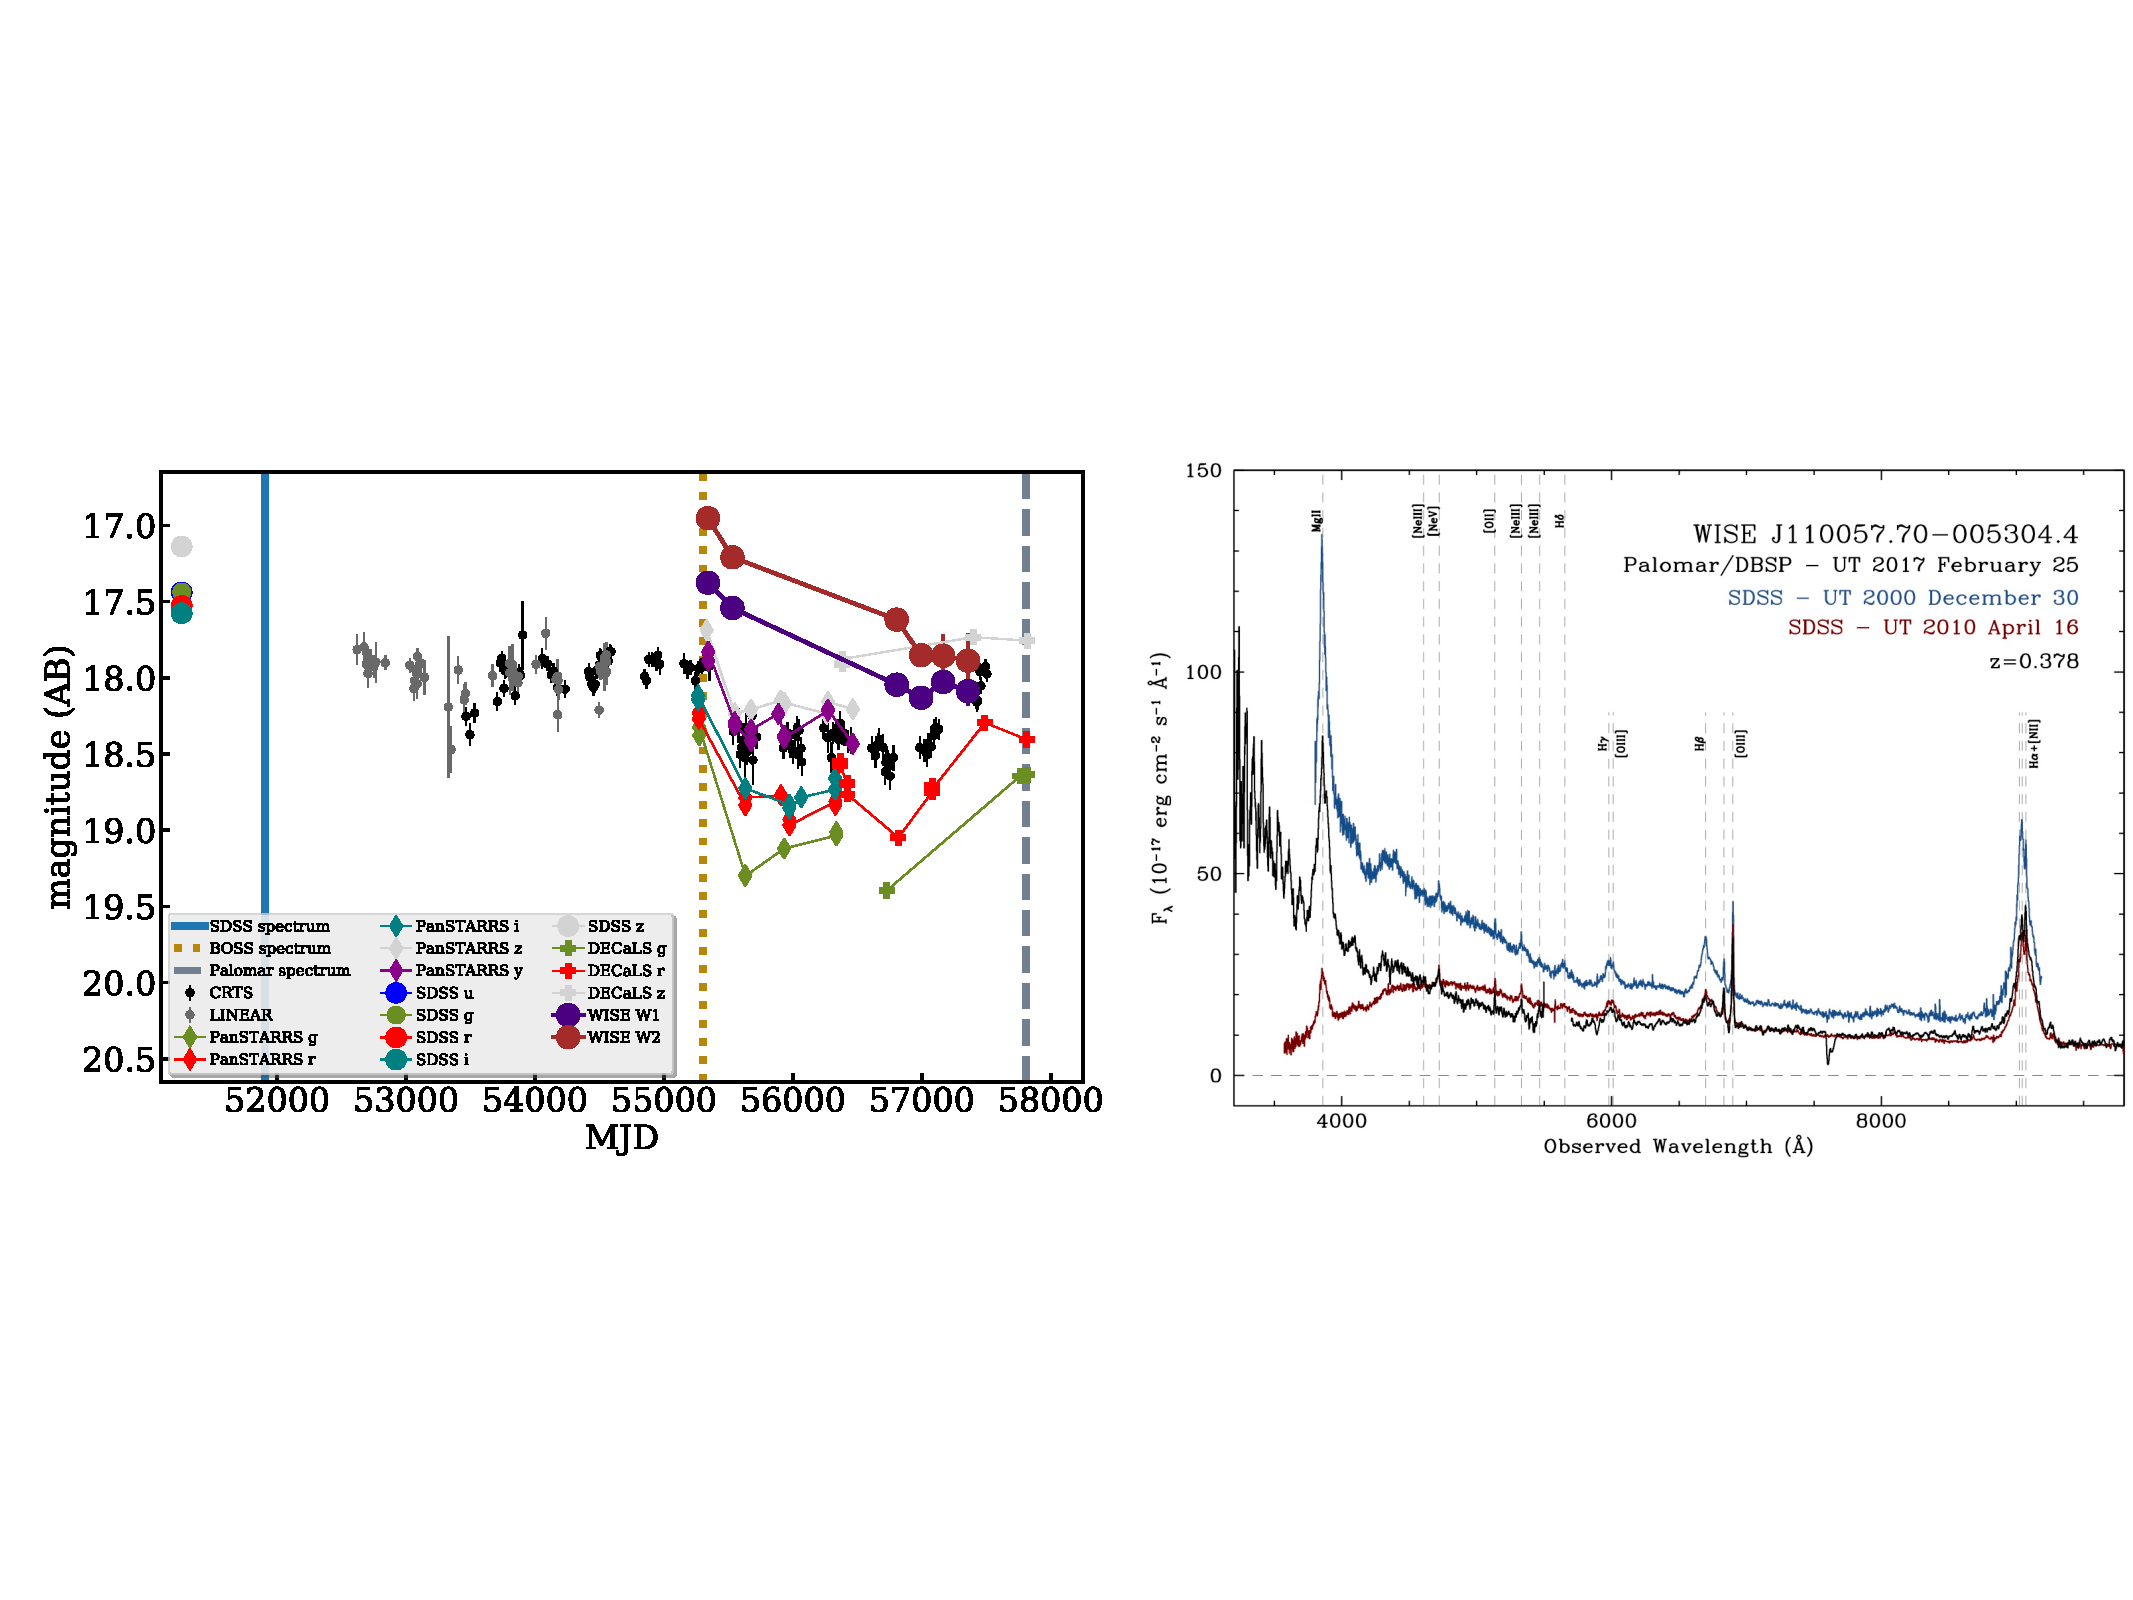
\includegraphics[height=6.25cm,width=17.2cm]
    {figures/J110057_LC_Spectra_20171024.pdf}
    \vspace{-10pt}
    \caption{%\small      
      \footnotesize 
      % \scriptsize
      % \tiny
      {\it (Left:)} The optical and infrared light-curve for J110057; 
      Note the fall in the infrared, whereas there is a decrease, but 
      then recovery in the optical. 
      {\it (Right:)} 
      Three epochs of spectra for J110057. 
      The spectacular downturn in the blue for the 2010 spectrum 
      indicates a dramatic change in the accretion disk.
    }
  \vspace{-16pt}
 \label{fig:J110057}
\end{center}
\end{figure}

\smallskip
\smallskip
\noindent
\textbf{\textsc{New IR investigations into the CLQ Population:}}
Taking advantage of new optical imaging data from the Dark Energy
Camera Legacy Survey \href{http://legacysurvey.org/decamls/}{(DECaLS)}
and new IR light-curves from NEOWISE ([26, 27]), we have made further
in-roads into understanding the CLQ population. This includes
identifying objects with rapidly changing IR light-curves and also
accretion disk changes, e.g. the $z=0.378$ quasar SDSS
J110057-005304.4, see Figure~\ref{fig:J110057}. From J110057, my new
model ([28]) suggests a dramatic new picture of the physics of the
CLQs governed by processes at the innermost stable circular orbit
(ISCO) and the structure of the innermost disk. {\it We have embarked
on a new observation campaign, gaining optical light-curves (from the
Liverpool Telescope) and spectra (from WHT and Palomar) to test this
startling new hypothesis.}



\smallskip
\smallskip
\noindent
%\textbf{\textsc{\textcolor{Cerulean}{Maximising Science Returns from European priorities:}}}
\textbf{\textsc{Maximising Science Returns from European priorities:}}
Contemporary astronomy is a multi-national endeavor with many leading
facilites being international collaborations. Although a project, with
similar but much less ambitious science goals and return could be
envisaged at the national level, the full discovery and break-through
nature being described herein only comes to the fore when the data
from the various international collaborations are combined
intelligently.  Critically data from leading European Southern
Observatory (ESO) and European Space Agency (ESA) facilites will play
a pivotal role here.

\smallskip
\smallskip
\noindent
One main ticket-item will be developing the {\it Event Broker Service}
that will interface with the e.g. LSST databases, pipelines and
transient stream. This is an already solved problem in many areas 
of DS and InfoSec, but we require a custom build in order to access 
the data streams necessary for our science goals. 


\smallskip
\smallskip
\noindent
%\subsection{Contemporary Galaxy formation theory}
\textbf{\textsc{Contemporary Galaxy formation theory:}}
The outstanding challenge in contempory galaxy formation theories is...

\smallskip
\smallskip
\noindent
{\bf COLORs....} In your first sentence start by giving some background information to the problem (to set the scene), you can also provide some statistics or financial information i.e. current cost of the disease to the health system, purification of water etc. Follow this by what is the current situation and what your ground breaking solution is to this problem. Does this need a coordinated effort across a number of different disciplines? Also stress here why you are uniquely placed to answer this problem.

\smallskip
\smallskip
\noindent
``State of the art is 43 objects, 11 of which I've discovered.''

%\subsection*{Facilities}
\begin{framed}
\begin{tcolorbox}
\begin{center} 
  Overview of Facilities and Surveys related to this propopsal
\end{center}
\end{tcolorbox}

The {\bf Sloan Digital Sky Survey (SDSS):} An ongoing project, currently in its fourth phase, SDSS-IV.  
The P.I. was a leading member of the SDSS-III: Baryon Oscillation Spectroscopic Survey (BOSS). 
The fifth generation of Sloan Digital Sky Surveys: SDSS-V will be an all-sky, multi-epoch spectroscopic 
survey, yielding spectra of over 6 million objects during its lifetime. Data taking is due to start in 
2020. Access would be through a USD \$230,000 'buy-in' (which allows access for the P.I. and one PDRAs).  . 
{\it Data Products: Repeat spectra in the North and Southern Hemisphere for 500,000 bright QSOs.} \\

The {\bf Dark Energy Spectroscopic Instrument (DESI) Survey:} is a 5 year cosmology survey 
that will be conducted on the Mayall 4-meter telescope at Kitt Peak National Observatory starting 
in 2019. It uses the 5,000 fiber Dark Energy Spectroscopic Instrument and will obtain optical 
spectra for $\approx$20 million galaxies and quasars. The DESI Survey is starts in late 2019 
and data access is through a USD \$250,000 `buy-in' (which allows access for the P.I. and two PDRAs).  \\
{\it Data Products: Spectra of 1e6 quasars across 14,000 deg$^{2}$ of the Northern Sky.} \\

\textit{\textbf{Euclid}} is an ESA Medium Class mission to map the geometry of the dark Universe.
It aims to understand why the expansion of the Universe is accelerating and what the nature 
of the source responsible for this acceleration (``dark energy'') is. 
%%
The
mission will investigate the distance-redshift relationship and the
evolution of cosmic structures by measuring shapes and redshifts of
galaxies and clusters of galaxies out to redshifts $\sim$2, or equivalently
to a look-back time of 10 billion years. In this way, Euclid will
cover the entire period over which dark energy played a significant
role in accelerating the expansion.
%%
{\it Euclid} is planned for launch in mid-2021. 
%%
{\it Data Products: Very broadband optical and 3 filter near-infrared space-based imaging for 15,000 deg$^2$.} \\

The {\bf Large Synoptic Survey Telescope (LSST)} project will conduct
a 10-year survey of the sky, imaging the full Southern Sky every 3
nights. The LSST survey is designed to address four science areas
(Understanding the Mysterious Dark Matter and Dark Energy; Hazardous
Asteroids and the Remote Solar System; The Transient Optical Sky; The
Formation and Structure of the Milky Way) and is an absolutely unique
facility as far as areal, temporal and wavelength coverage.\\
{\it Data Products: $ugrizY$ broadband optical and near-infrared imaging for 20,000 deg$^2$. 
Images the full Southern Sky every 3 days. } \\

The {\bf 4-metre Multi-Object Spectroscopic Telescope  (4MOST):} 
is a fibre-fed spectroscopic survey facility on the VISTA telescope with a large enough field-of-view to survey a large fraction of the southern sky. The facility will be able to simultaneously obtain spectra of 2,400 objects distributed over a field-of-view of 4 square degrees. 
The initial Galactic and Extragalactic surveys will operate over a five-year period delivering spectra for $\geq$25 million objects over 
$\gtrsim$15,000 deg. 4MOST will commence science operations in mid-2021 ({\bf TO BE CHECKED!!!}. 
{\it Data Products: } \\

{\underline Notes::} 4MOST has full access to the full LSST footprint. LSST will overlap half (7,500 deg$^2$) of the {\it Euclid} footprint. \\

The {\it Extended Roentgen Survey with an Imaging Telescope Array (eROSITA)} is the main instrument on the 
Spektr-RG (Spectrum-X-Gamma; SRG, SXG), an international high-energy astrophysics observatory. 

\hrulefill 

The {\bf Wide-field Infrared Survey Explorer (WISE)} is a NASA
infrared-wavelength astronomical space telescope launched in December
2009 and is still operation (in its ``NEOWISE-R'' mission phase as at
the time of writing). WISE performed an all-sky astronomical survey
with images at 3.4, 4.6, 12 and 22$\mu$m using a 40cm (16 in) diameter
infrared telescope in Earth orbit. 

The {\bf James Webb Space Telescope (JWST)} is a space telescope
developed in coordination among NASA, the European Space Agency, and
the Canadian Space Agency. It is scheduled to be launched in June
2019. The telescope will offer unprecedented resolution and
sensitivity from 0.6 to 27$\mu$m.
%%
JWST is a partnership between NASA, ESA and the Canadian Space Agency.
In particular, ESA's contributions to JWST include (but are not
limited to) the NIRSpec instrument and the Optical Bench Assembly of
the MIRI instrument.  In return for these contributions, ESA gains
full partnership in JWST and secures full access to the JWST
observatory for astronomers from ESA Member States on identical terms
to those of today on the Hubble Space Telescope. European scientists
will be represented on all advisory bodies of the project and will be
expected to win observing time on JWST through a joint peer review
process, backed by an expectation of a minimum ESA share of 15\% of
the total JWST observing time.


The ESA {\it Gaia} mission is an ongoing mission to chart a
three-dimensional map of our Galaxy, the Milky Way, in the process
revealing the composition, formation and evolution of the Galaxy. Gaia
is providing unprecedented positional and radial velocity measurements
with the accuracies needed to produce a stereoscopic and kinematic
census of about $\sim$one billion stars in our Galaxy and throughout
the Local Group. This amounts to about 1 per cent of the Galactic
stellar population.
%\hline 
%\hline
\end{framed}

%%sizes and timescales:: \\
%%10$^{8}$ MBH to Jupiter, \\
%%speed at which we send a probe there...\\



\subsection*{2. Objectives}

%\smallskip \smallskip
\noindent
The objectives of the proposal are:
\begin{itemize}
\item To elucidate on how the energetics of the galaxy central engine impact the host galaxy;
\item To produce the state-of-the-art (and quite possibly the unique) multi-wavelength, multi-epoch 
quasar dataset from the combination of 5 of the worlds leading surveys in 2020; 
\item To connect, for the first time, the physical mechanisms acting on sub-parsec to mega-parsec scales. 
\end{itemize}

\smallskip
\smallskip
\noindent
This will be achieved by:
\begin{itemize}
\item Characterizing one million changing look quasars;
\item Cataloging {\it Euclid}, 4MOST, SDSS-V, DESI and LSST quasars; 
\item Theoretically connecting new simulation codes at the accretion disk and galaxy-scales. 
\end{itemize}

\smallskip
\smallskip
\noindent
Some points to keep in mind when include::
\begin{itemize}
\item clearly state why and how the proposed work is novel and important in your field
\item what are your objectives,
\item What are the key challenges/open questions in your field that need to be answered 
\item how will you go about it, clearly explain how you propose to address these questions. 
\item what are the expected outcomes?
\item  explain the impact of your work- if you are successful-, on the research area and beyond and your long term vision.
\end{itemize}

